\subsection{System 8 Binned Results}

Here we show the measured b-tag efficiency from System8 compared to the 
expected efficiency from MC truth information as a function of jet $p_{T} $.
Figure~\ref{fig:S8_TC_results}shows the results for the Track Counting
algorithm for the three operating points (loose,medium and tight) and also the 
SLT results using the default Track 
Counting algorithm. Only the statistical errors are shown and we observe a 
reasonably good agreement in measured and expected efficiencies. In 
Figure~\ref{fig:S8_JP_results} are shown the measured
b-tag efficiencies from System8 compared to the expected for the loose,medium 
and tight operating points for the Jet Probability tagger. The results are 
shown for the $pp\rightarrow \mu + X$ sample which has a lower number of light 
jets so the correlation factors for light jets have large uncertainty. This is 
reflected in the Jet Probability tagger which seems to be more senstive to this
effect.

\begin{figure}[htbp]
  \begin{center}
    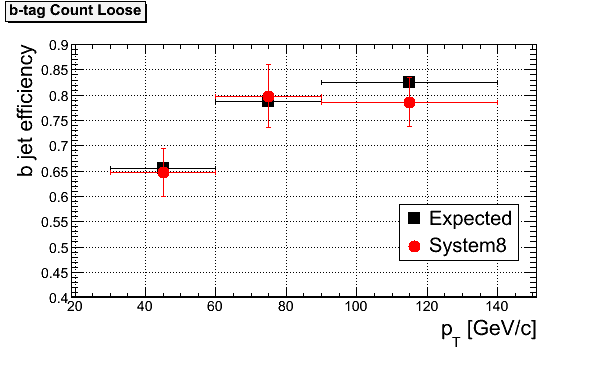
\includegraphics[width=70mm]{Figures/TCL_Tag.png}
    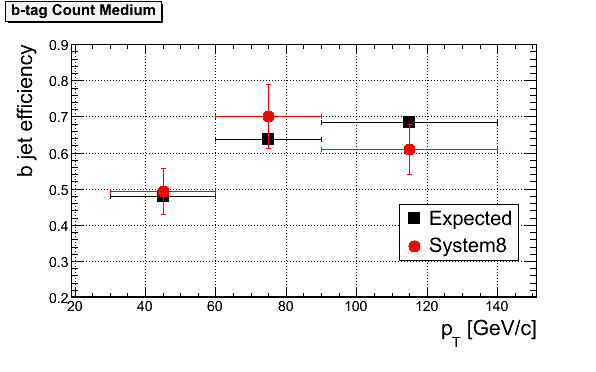
\includegraphics[width=70mm]{Figures/TCM_Tag.png}
    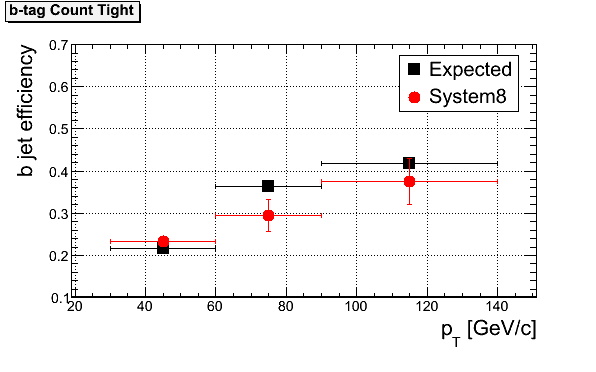
\includegraphics[width=70mm]{Figures/TCT_Tag.png}
    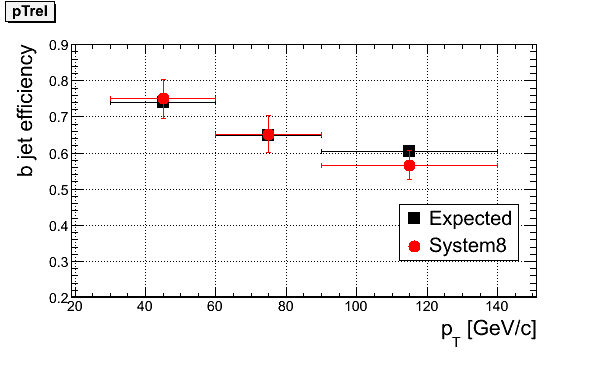
\includegraphics[width=70mm]{Figures/pTrel.png}
  \end{center}
  \caption{Measured and expected b$-$tag efficiency from System8 for the 
$pp\rightarrow \mu+ X$ sample as a function of jet $p_T $ 
(requiring $p_T $ $> $ 30 GeV/c).The error bars shown are only statistical 
errors.}
  \label{fig:S8_TC_results}
\end{figure}
\vspace{-5cm}

\begin{figure}[htbp]
  \begin{center}
    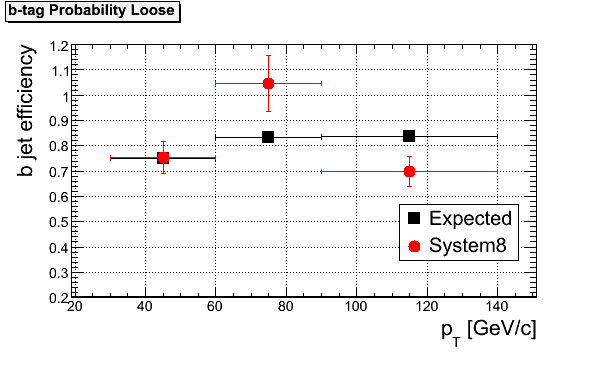
\includegraphics[width=70mm]{Figures/JPL_Tag.png}
    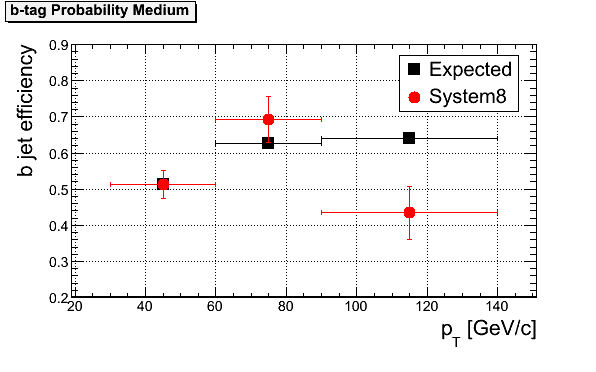
\includegraphics[width=70mm]{Figures/JPM_Tag.png}
    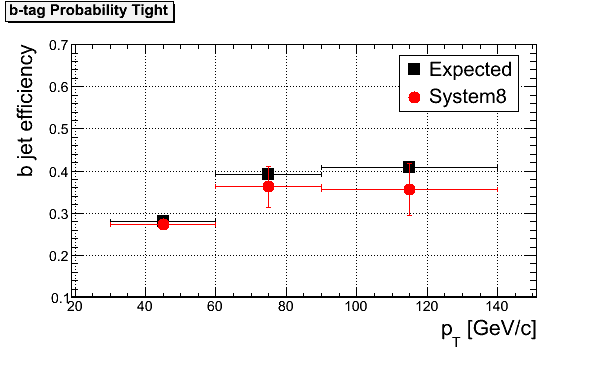
\includegraphics[width=70mm]{Figures/JPT_Tag.png}
  \end{center}
  \caption{Measured and expected b$-$tag efficiency from System8 for the
$pp\rightarrow \mu +X $ as a function of jet $p_T $ 
(requiring $p_T $ $> $ 30 GeV/c). The error bars shown are only statistical 
errors.}
  \label{fig:S8_JP_results}
\end{figure}

\clearpage

